\chapter{Experimentálna časť}


\section {Ciele epxerimentu}

V oblasti Q-learning algoritmoch je možné pozorovať dva hlavné smery výskumu

\begin{itemize}
\item aproximácia funkcie ohodnotení
\item spôsob výberu akcie
\end{itemize}

Obe majú široké pole diskusií v snahe vyriešit niekoľko hlavných problém Q-learning
algoritmu a to najmä

\begin{itemize}
\item veľký počet prechodov medzi stavmi
\item malá zmena vo výpočte $Q(s(n),a(n))$ môže spôsobiť veľké zmeny v stratégií.
\end{itemize}

Cieľom práce je na danej množine odmeňovacích funkcií $R(s(n), a(n))$ overiť
možnosti aproximácie $Q(s(n), a(n))$.
V niekoľkých bodoch je možné postup určiť ako

\begin{itemize}
\item výber funkcií $R(s(n), a(n))$
\item určenie presného riešenia, použitím tabuľky s veľkým počtom prvkov
\item voľba aproximačnej metódy
\item pre každú $R(s(n), a(n))$ spočítať niekoľko nezávislych behov
\item výsledky porovnať s presným riešením, overiť a zosumarizovať
\end{itemize}

Funkcie $R(s(n), a(n))$ budu vybrané tak aby boli riedke a plne sa využil Q-learing -
okamžité odmeny sú známe len v malom počte prípadov.
Postupne sa obmenia pre rôzne počty nenulových prvkov.

Presné riešenie, aby bolo možné spočítať bude mať niekoľko tisíc diskrétnych stavov.
Pre jednoduchosť, bude v každom stave rovnaká a presne definovaná množina akcií.

Vyberie sa niekoľko aproximačných metód, ktoré sa použijí na spočítanie $Q(s(n), a(n))$.
Tu je nevyhnutné upozorniť na častú metodickú chybu : aj keď je možné $Q(s(n), a(n))$
spočítať presne, nesmie byť toto presne riešenie použité na stanovenie približného riešenia.
Príkladom je dopredná neurónová sieť, ktorá sa dá veľmi ľahko natrénovať ak je množina požadovaných
výstupov vopred známa. V prípade Q-learning algoritmu sa ale požadované hodnoty spočítavajú
rekuretne, až počas behu.

Kedže voľba niektorých počiatočných parametrov aproximačných metód je náhodná,
je nevyhnutné spočítať niekoľko nezávislých behov a overť tak rozptyl, minimálnu, maximálnu
a priemernu chybu.

\section {Návrh experimentu}

Aby sa dalo kvalitatívne ohodnotiť použité riešenie, je nutné urobiť veľký počet experimentov.
Aby bolo možné ľahko graficky znázorniť výsledok, bude stavový priestor dvojrozmerný a platí
$s(n) \in \langle -1, 1 \rangle$.
Agent si bude vyberať z pevne danej množiny akcií a bude sa tak v tomto priestore môcť pohybovať a to :

$\mathbb{A} = [ [0, 1], [0, -1], [1,  0], [-1, 0], [1, -1], [1, 1], [-1, -1], [-1, 1]] $

prostredie umožní zmenu stavu vykonaním akcie $a(n) \in \mathbb{A}$, a to podľa

\begin{equation}
s(n+1) = s(n) + a(n){dt}
\label{eq:q_learning}
\end{equation}

Jednotlivé funkcie $R^k(s(n), a(n))$ predstavujú mapy odmien v ktorých sa agent pohybuje. Pre zjednodušenie
bude platiť, že nezáleží ktorou akciou sa agent dostal do daného stavu - funkcia bude
mať teda tvar $R^k(s(n))$ a predstavuje teda odmenu za to, že sa agent dostal na nejaké miesto.

Ako metódy aprximácie je zvolených 5 rôznych funkcií.

\begin{enumerate}
\item riedka tabuľka
\item Gaussova krivka $f_j^1(\boldmath{s(n), a(n)})$ \ref{eq:basis_functions}
\item Gaussova krivka $f_j^1(\boldmath{s(n), a(n)})$ kombinovaná s riedkou tabuľkou
\item Modifikácia Kohonenovej neurónovej siete $f_j^2(\boldmath{s(n), a(n)})$
\item Modifikácia Kohonenovej neurónovej siete $f_j^2(\boldmath{s(n), a(n)})$ s riedkou tabuľkou
\end{enumerate}

Pre každú z nich prebehne 20 trialov aby bolo možné urobiť štatistické vyhodnotenie.
V každom trialy prebehne 10*50000 učiacich interácií aby bolo možné v 10 tich krokoch sledovať
priebeh učenia. Na konci prebehne 50 behov agentov z náhodných východzich stavov aby bolo
možné sledovať ich cestu stavovým priestorom.

\begin{figure}[!htb]
\center
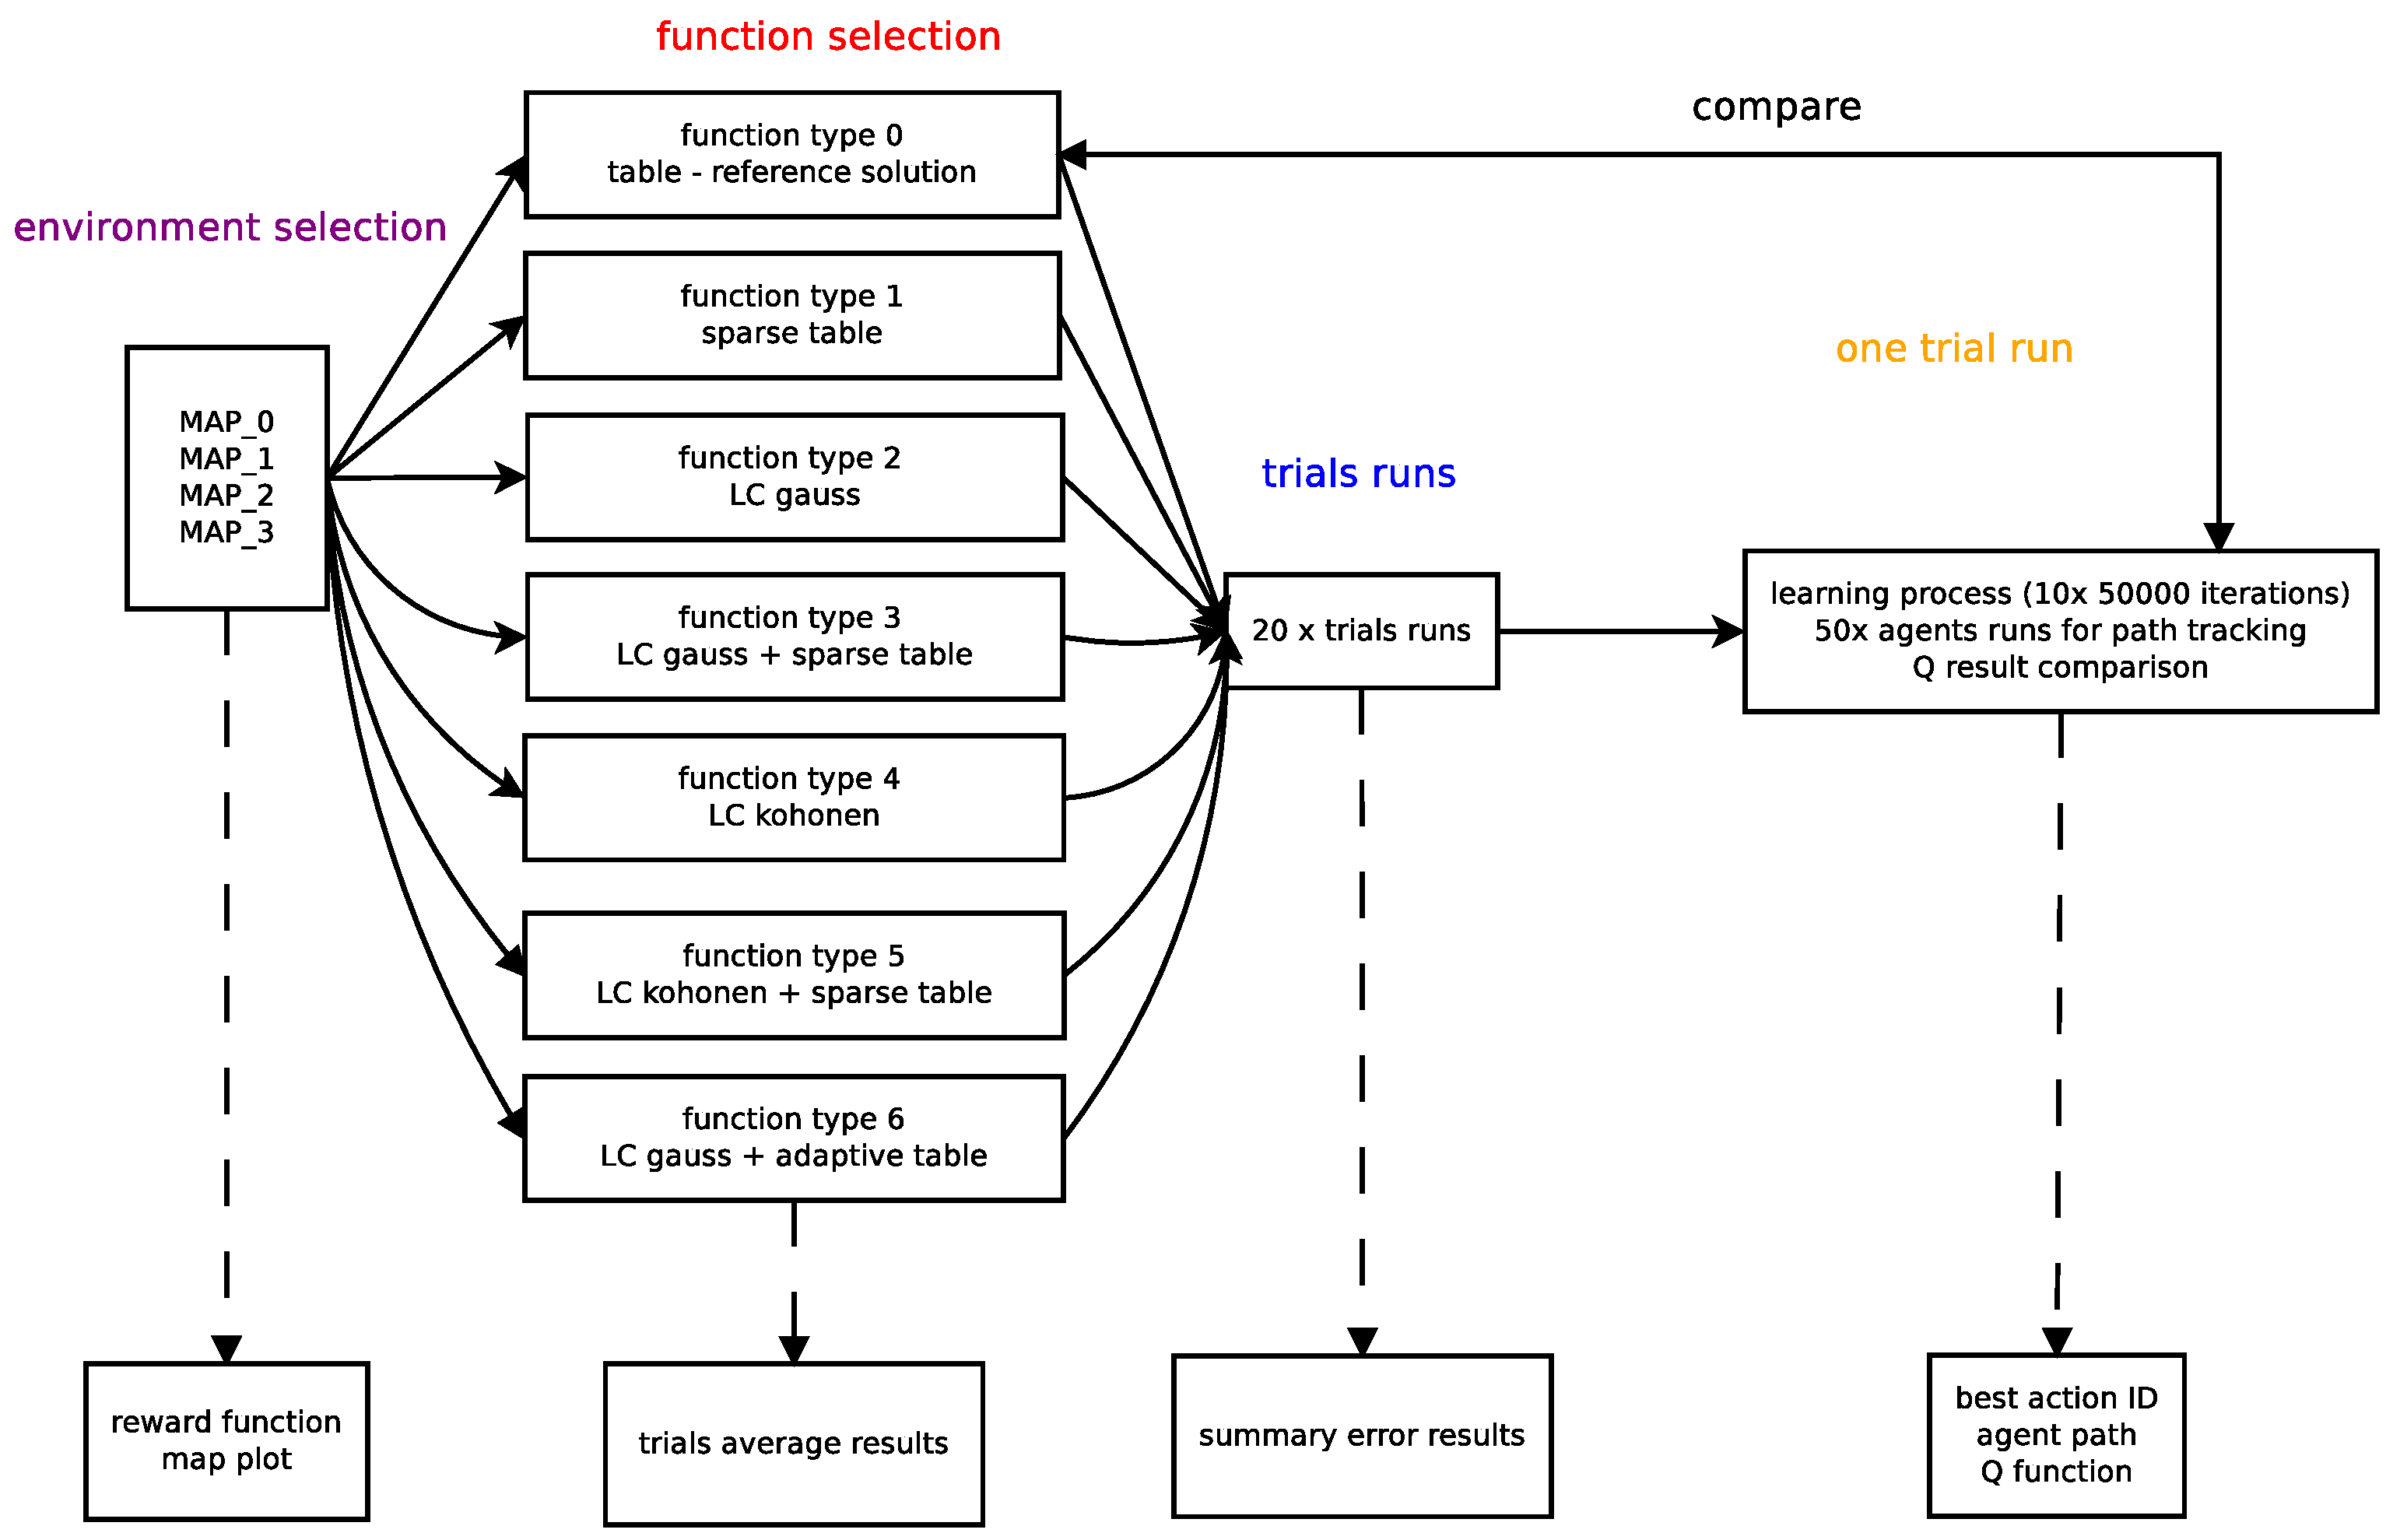
\includegraphics[scale=.3]{../diagrams/experiment_map_q_learning.eps}
\caption{Schéma experimentu}
\label{img:experiment_schem}
\end{figure}

Súhrnná schéma behu experimentov je na obrázku \ref{img:experiment_schem}.
Plné šípky predstavujú prepojenie úrovni metodológie. Čiarkované šípky znázorňujú
výstupy v jednotlivých úrovniach. Presné riešenie je použité na porovnanie výslednej chyby.



\begin{itemize}
\item 50000 iterácií učenia
\item rozmer $s$ je $n_s = 2$, rozmer $a$ je $n_a = 2$
\item predpis funkcie ohodnotení
\begin{align}
&Q(s(n),a(n)) = \nonumber \\
&\alpha Q(s(n-1),a(n-1)) \nonumber \\
&(1- \alpha)(R(s(n),a(n)) + \gamma \max_{a(n-1) \in \mathbb{A}} Q(s(n-1), a(n-1)) \nonumber
\end{align}

\item $R(s(n), a(n)) \in \langle -1, 1 \rangle$ náhodná mapa s 1 cieľovým stavom
\item $\gamma = 0.98$ a $\alpha = 0.7$
\item hustota referenčného riešenia = 1/32  (4096 stavov)
\item počet akcií v každom stave = 8
\item hustota riedkej tabuľky = 1/8  (1:16 pomer)
\item počet bázických funkcií $l = 64$
\item rozsah parametrov
    \begin{itemize}
      \item $\alpha_{ja}(n) \in \langle -1, 1 \rangle$
      \item $\beta_{ja}(n) \in \langle 0, 200 \rangle$
      \item $w_{ja}(n) \in \langle -4, 4 \rangle$
    \end{itemize}
\end{itemize}

$Q_{rt}(s(n),a(n))$ referenčná funkcia Q (funkcia 0), kde $t \in \langle 0, 19 \rangle $ je číslo trialu  \\
$Q_{jt}(s(n),a(n))$ testované funkcie Q a $j \in \langle 1, 5 \rangle $. \\

Celková chyba behu trialu $t$ je \\
\begin{equation}
e_{jt} = \sum\limits_{s, a}{(Q_{rt}(s,a) - Q_{jt}(s,a))^2}  \nonumber
\end{equation}

priemerná, minimálna, maximálna chyba a smerodatná odchylka \\
\begin{align}
\bar{a_j} &= \frac{1}{20}\sum\limits_{t}{e_{jt}}  \nonumber \\
{e^{min}_j} &= \min_{t}{e_{jt}}  \nonumber \\
{e^{max}_j} &= \max_{t}{e_{jt}}  \nonumber \\
{\sigma_j}^2 &= \frac{1}{20}\sum\limits_{t}{(\bar{a_j} - e_{jt})^2}  \nonumber
\end{align}

\section {Výsledky experimentu}



\begin{figure}[!htb]
\centering
\includegraphics[scale=.4]{../../results_q_learning/map_1/reward_value_surface.png}
\caption{odmeňovacia funkcia}
\end{figure}



\begin{figure}[!htb]
\centering
\includegraphics[scale=.4]{../../results_q_learning/map_1/function_type_1/iterations_10/action_best_value_log_surface.png}
\caption{fig:sparse table}
\end{figure}

\begin{figure}[!htb]
\centering
\includegraphics[scale=.4]{../../results_q_learning/map_1/function_type_2/iterations_10/action_best_value_log_surface.png}
\caption{fig:linear combination Gauss}
\end{figure}




\begin{figure}[!htb]
\includegraphics[scale=.4]{../../results_q_learning/map_1/function_type_3/iterations_10/action_best_value_log_surface.png}
\caption{sparse table + linear combination Gauss}
\end{figure}


\begin{figure}[!htb]
\includegraphics[scale=.4]{../../results_q_learning/map_1/function_type_4/iterations_10/action_best_value_log_surface.png}
\caption{linear combination Kohonen function}
\end{figure}




\begin{equation}
e_{jt}(s) = (Q_{rt}(s,a - Q_{jt}(s,a))^2  \nonumber
\end{equation}


\begin{figure}[!htb]
\centering
\includegraphics[scale=.4]{../../results_q_learning/map_1/function_type_1/q_learning_error.png}
\caption{sparse table}
\end{figure}


\begin{figure}[!htb]
\centering
\includegraphics[scale=.4]{../../results_q_learning/map_1/function_type_2/q_learning_error.png}
\caption{linear combination Gauss}
\end{figure}



Chybové funkcie - Výsledky experimentov

\begin{equation}
e_{jt}(s) = (Q_{rt}(s,a - Q_{jt}(s,a))^2  \nonumber
\end{equation}

\begin{figure}[!htb]
\centering
\includegraphics[scale=.4]{../../results_q_learning/map_1/function_type_3/q_learning_error.png}
\caption{sparse table + linear combination Gauss}
\end{figure}



\begin{figure}[!htb]
\centering
\includegraphics[scale=.4]{../../results_q_learning/map_1/function_type_4/q_learning_error.png}
\caption{linear combination Kohonen function}
\end{figure}






max Q(s, a) - Výsledky experimentov


\begin{figure}[!htb]
\centering
\includegraphics[scale=.4]{../../results_q_learning/map_1/function_type_0/iterations_10/q_learning_result.png}
\caption{reference table}
\end{figure}


\begin{figure}[!htb]
\centering
\includegraphics[scale=.4]{../../results_q_learning/map_1/function_type_3/iterations_10/q_learning_result.png}
\caption{sparse table + linear combination Gauss}
\end{figure}




Priebeh trialov - Výsledky experimentov

\begin{figure}[!htb]
\centering
\includegraphics[scale=.4]{../../results_q_learning/map_1/trials_average_results_progress.png}
\end{figure}




Mapa 1 - Výsledky experimentov

\begin{figure}[!htb]
\centering
\includegraphics[scale=.4]{../../results_q_learning/map_1/trials_average_results.png}
\end{figure}



Mapa 0 - Výsledky experimentov

\begin{figure}[!htb]
\centering
\includegraphics[scale=.4]{../../results_q_learning/map_0/trials_average_results.png}
\end{figure}


Mapa 2 - Výsledky experimentov

\begin{figure}[!htb]
\centering
\includegraphics[scale=.4]{../../results_q_learning/map_2/trials_average_results.png}
\end{figure}


Mapa 3 - Výsledky experimentov

\begin{figure}[!htb]
\centering
\includegraphics[scale=.4]{../../results_q_learning/map_3/trials_average_results.png}
\end{figure}
